% \chapter{Funktion einer CMDB im RZ-Umfeld}
% \newpage \setcounter{page}{11} %Seitenzähler zurücksetzen
\chapter{Anforderungsanalyse anhand von Experteninterviews} \label{AnfA}
% In diesem Kapitel wird
Um die Anforderungen an einen \acs{CMDB} Chatbot zu erfassen, wird in diesem Kapitel eine Anforderungsanalyse nach Pohl und Rupp durchgeführt, die als Werkzeug zur Anforderungsermittlung das Experteninterview nach Meuser und Nagel verwendet.

Ziel des Anforderungsmanagements bzw. Requirements Engineerings nach Pohl und Rupp ist die Erfassung und Dokumentation von Anforderungen.\footcite[Vgl.][3]{Pohl_2015_Requirements}

Wesentliche Funktionen des Experteninterviews sind Informationsgewinnung und Theorieentwicklung, weswegen es sich als Methode eignet, um Anforderungen zu erheben.
\footcites[Vgl.][9]{Bogner_2014_Interview}[Vgl.][187\psq]{Glaeser_2010_Inhaltsanalyse}

Wenn von Experteninterviews die Rede ist, kann man davon ausgehen, dass ein leitfadengestütztes, qualitatives Interview gemeint ist. Da das Instrument Experteninterview dem Forschungsvorhaben angepasst werden muss, können jedoch verschiedene Dinge unter dem Begriff verstanden werden und es ist nötig klarzustellen, welche Ausprägung gemeint ist.\footcite[Vgl.][3]{Bogner_2014_Interview}
Auch der Expertenbegriff muss der Forschungsfrage angepasst werden.\footcite[Vgl.][180]{Meuser_1994_Interview}

In dieser Arbeit wird der qualitativ ausgerichtete Ansatz von Meuser und Nagel angewendet. Quantitative Ansätze oder qualitative Ansätze anderer Autoren, die von dem behandelten abweichen werden hier nicht weiter ausgeführt.\footcite[Vgl.][o. \pno]{Meuser_2010_Interview}

Meuser und Nagel unterscheiden Experteninterviews grundlegend in systematisierende und explorativ-felderschließende Interviews. Bei ersteren wird der Experte zu seinem eigenen Fachgebiet befragt (Betriebswissen), bei letzerem liefert er \glqq{}Informationen über die Kontextbedingungen des Handelns der Zielgruppe\grqq\footcite[][445]{Meuser_1991_Interview} (Kontextwissen).\footcite[Vgl.][445]{Meuser_1991_Interview}

Bogner, Littig und Menz sprechen in diesem Zusammenhang von fundierenden und explorativen Interviews und fassen die vormals genannten Kategorien unter dem Begriff \textit{informatorisch} zusammen. Außerdem ergänzen sie zwei  deutungswissenorientierte Varianten. Eine genaue Aufschlüsselung ist in \autoref{tab:artenei} zu sehen.
\footcites[Vgl.][22\psqq]{Bogner_2014_Interview}[Vgl.][445\psq]{Meuser_1991_Interview}


\begin{table}[H]
\centering
\begin{tabularx}{1\textwidth}{l|X|X}
                            & Explorativ (Kontextwissen) & Fundierend (Betriebswissen) \\\hline
   Informatorisch           & Explorative Datensammlung & Systematisierendes Interview \\
   Deutungswissenorientiert & Exploration von Deutungen & Theoriegenerierendes Interview\\
\end{tabularx}
  \quelleeigen[22\psqq]{Bogner_2014_Interview}[445\psqq]{Meuser_1991_Interview}
\caption{Arten von Experteninterviews}
\label{tab:artenei}
\end{table}

%\begin{table}[H]
%\centering
%\begin{tabularx}{1\textwidth}{|l||X|X|}\hline
%                            & Explorativ (Kontextwissen) & Fundierend (Betriebswissen) \\\hline\hline
%   Informatorisch           & Explorative Datensammlung & Systematisierendes Interview \\\hline
%   Deutungswissenorientiert & Exploration von Deutungen & Theoriegenerierendes Interview\\\hline
%\end{tabularx}
%  \quelleeigen[22\psqq]{Bogner_2014_Interview}[445\psqq]{Meuser_1991_Interview}
%\caption{Arten von Experteninterviews}
%\label{tab:artenei}
%\end{table}



 Als Interviewart wird in dieser Arbeit das \textit{informatorische Interview}, genauer gesagt die \textit{explorative Datensammlung} genutzt, um von den Experten \textit{Kontextwissen} abzufragen.

Anforderungen werden dabei als Aussagen über Leistungen oder Fähigkeiten, die von einem System zu erbringen sind und die entsprechenden zur Zielerreichung nötigen Eigenschaften verstanden.\footcite[Vgl.][3]{Pohl_2015_Requirements}

Die Haupttätigkeiten der Anforderungsanalyse sind die Ermittlung, Dokumentation, Prüfung und Verwaltung von Anforderungen, wobei die Verwaltung mit den drei vorigen Tätigkeiten einher geht. \footcite[Vgl.][4\psq]{Pohl_2015_Requirements}

Ein Experteninterview kann aus bis zu acht Phasen bestehen. Der Leitfadenerstellung, Tonaufnahme, Transkription, Paraphrase, (Bildung von) Überschriften, dem thematischen Vergleich, der soziologischen Konzeptualisierung und theoretischen Generalisierung.
Da Kontextwissen und nicht Betriebswissen abgefragt wird, empfehlen Meuser und Nagel, das Experteninterview mit dem thematischen Vergleich abzuschließen und die letzten beiden Phasen entfallen zu lassen. Es wird also in diesem Fall keine soziologische Konzeptualisierung und theoretische Generalisierung durchgeführt. \footcite[Vgl.][466\psq]{Meuser_1991_Interview}

Die Phasen und Parallelen von Anforderungsanalyse und Experteninterview sind in einer Übersicht in \autoref{tab:expanf} dargestellt.

%\begin{table}[H]
%\centering
%{
%\setlength\tabcolsep{1.5pt}
%\setlength\extrarowheight{2pt} %new code
%% \def\arraystretch{1}%
%\begin{tabularx}{1\textwidth}{|p{1cm}|X|X|}\hline
%& Anforderungsanalyse & Experteninterview\\\hline
% \multicolumn{1}{|c|}{\multirow{-0.5}{*}{\RotText{4. Verwaltung}}} & 1. Ermittlung & 1. Leitfadenerstellung \newline 2. Tonaufnahme \\\cline{2-3}
%  \multicolumn{1}{|c|}{} & 2. Dokumentation & 3. Transkription \newline 4. Paraphrase \newline 5. Überschriften \\\cline{2-3}
%  \multicolumn{1}{|c|}{} & 3. Prüfung und Abstimmung & 6. Thematischer Vergleich \\\cline{1-3}
%  & & \sout{7. Soziologische Konzeptualisierung} \newline \sout{8. Theoretische Generalisierung}\\\hline
%\end{tabularx}
%}
%  \quelleeigen[466\psq]{Meuser_1991_Interview}[4\psq]{Pohl_2015_Requirements}
%\caption{Experteninterview und Anforderungsmanagement im Vergleich}
%\label{tab:expanf}
%\end{table}

\begin{table}[htbp]
\centering
{
\setlength\tabcolsep{1.5pt}
\setlength\extrarowheight{2pt} %new code
% \def\arraystretch{1}%
\begin{tabularx}{.8\textwidth}{p{1cm}X|X}
& Anforderungsanalyse & Experteninterview\\\hline
 \multicolumn{1}{c}{\multirow{-0.5}{*}{\RotText{4. Verwaltung}}} & 1. Ermittlung & 1. Leitfadenerstellung \newline 2. Tonaufnahme \\
  \multicolumn{1}{c}{} & 2. Dokumentation & 3. Transkription \newline 4. Paraphrase \newline 5. Überschriften \\
  \multicolumn{1}{c}{} & 3. Prüfung und Abstimmung & 6. Thematischer Vergleich \\
  & & \sout{7. Soziologische Konzeptualisierung} \newline \sout{8. Theoretische Generalisierung}\\
\end{tabularx}
}
\caption{Experteninterview und Anforderungsmanagement im Vergleich}
\label{tab:expanf}
\end{table}





\section{Aktuelle Situation}
Das \acs{IVZ} verwendet die \textit{i-doit} \acs{CMDB} des Herstellers synetics in dreistufiger Ausführung, also Entwicklung, Integration und Produktion.
Sämtliche Hardware wie Server, Infrastruktur (\acf{LAN}, \acf{SAN} Switche usw.) und Verkabelung sind in dieser \acs{CMDB} erfasst.\\
Auch Clients wie Computer und Laptops sowie mobile Endgeräte wie Tablets und Smartphones werden in die \acs{CMDB} eingetragen.\\
Virtuelle Maschinen und Cluster sind ebenfalls in der \acs{CMDB} hinterlegt.

Neben Hardware werden auch Softwarelizenzen, Wartungsverträge, \acfp{SLA} und der \acf{ITIL} Servicekatalog abgebildet. Dadurch können auslaufende Lizenzen und Verträge rechtzeitig erkannt und verlängert oder erneuert werden.\\
Beim Anlegen von virtuellen Maschinen oder Hardware Servern kann direkt der entsprechende Service oder Wartungsvertrag verknüpft werden. So entsteht auch ein Überblick darüber, welche Hardware wann aus der Wartung läuft und zu welchem Grad das Lizenzkontigent erschöpft ist. Gleiches gilt für Clients und deren Betriebssystem und etwaige installierte, lizenzpflichtige Software.

Auch \acf{DNS} Einträge und Layer-2 und 3 Netze sind in der \acs{CMDB} dokumentiert. Beim Anlegen oder Planen eines neuen Servers (physikalisch oder virtuell) können so direkt ein Hostname und eine IP-Adresse reserviert werden, bevor die Eintragung im \acs{DNS}-Server erfolgt. Das entsprechende User Interface ist in \autoref{fig:idoitip} zu sehen. Etwaige Konflikte fallen so frühzeitig auf, z. B. durch Ping, Lookup oder Reverse Lookup der gewünschten Adressen aus der IP Liste heraus kann die Verfügbarkeit der Adressen überprüft werden, wobei bestimmte Bereiche pro Netz der Infrastruktur vorbehalten sind.

\begin{figure}[H]
  \centering
  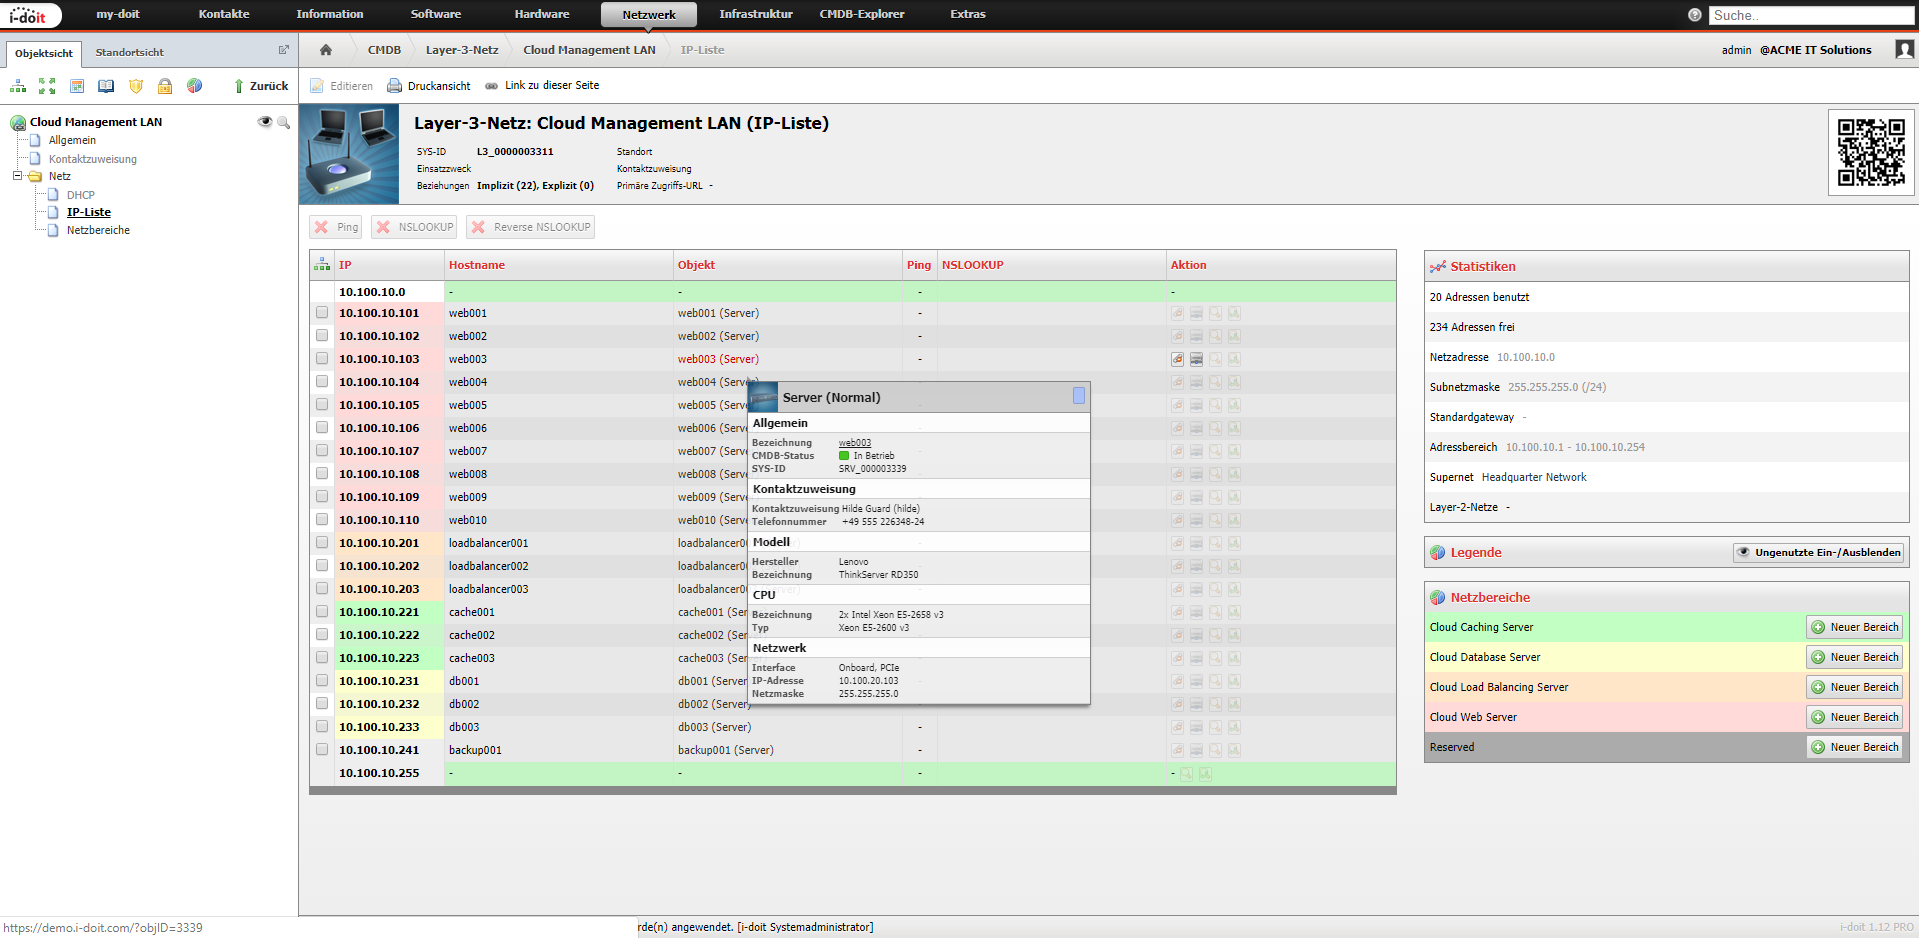
\includegraphics[width=\textwidth]{Anhang/idoitip}
  \quelle[o. \pno]{idoit_2019_idoitip}
  \caption{i-doit IP Management}
\label{fig:idoitip}
\end{figure}

Die \acs{CMDB} wird überwiegend vom Team \textit{Rechenzentrum} über das Webinterface verwendet. Wenn z. B. ein neuer Server angefordert wird, erfolgt die Planung von Hostname und IP-Adresse in der \acs{CMDB}.\\
Auch beim Einbau von Hardware, z. B. neuen Servern, wird die \acs{CMDB} prozessvorbereitend, -begleitend und -unterstützend eingesetzt: Es kann vorab geprüft werden, in welchen Racks noch genug Platz ist und wo entsprechende Möglichkeiten zur Verkabelung von Strom und Netzwerk bestehen. Wenn geprüft wurde, ob Kabel in der benötigten Länge vorrätig sind, kann der Einbau erfolgen und der Status der Hardware wird von \textit{geplant} auf \textit{in Betrieb} geändert.\\
Die verwendeten Kabel werden ebenfalls dokumentiert und die entsprechenden Knotenpunkte (z. B. Netzwerkkartenport zu Switchport oder Netzteil zu Steckerleiste) verknüpft.

Um die \acs{CMDB} von der Kommandozeile aus verwenden zu können, besteht die Möglichkeit, \textit{i-doit-cli} zu nutzen, einen \acf{API}-Client für die i-doit \acs{CMDB}.\\
Mit dem Client lassen sich z. B. Objekte suchen, Details dazu anzeigen und freie IP-Adressen in einem bestimmten Netz anzeigen. Um diese Operationen zu beschleunigen wird ein lokales Caching verwendet.\\
Außerdem können Dummy Einträge erzeugt werden, um die System-Performance zu testen. Der Client wird bisher nur in einigen Skripten verwendet und hat für die manuellen Tätigkeiten der Mitarbeiter keine Relevanz.
\footcite[Vgl.][o. \pno]{Heisig_2019_idoitcli}

Als Chat-Tool wird derzeit Slack eingesetzt, allerdings ist die Migration nach Cisco Webex Teams geplant. 


\section{Expertenauswahl}
Um das Experteninterview anwenden zu können, muss geklärt werden, wer als Experte gilt, was Expertenwissen bedeutet und wie man es abruft.\footcite[Vgl.][6\psq]{Bogner_2014_Interview}

\subsection{Kriterien}
Das Wort \textit{Experte} leitet sich aus dem lateinischen \textit{expertus} (erprobt, bewährt) ab, welches wiederum aus dem passiven Verb \textit{experiri} (prüfen, ausprobieren) gebildet wird. Experten sind also Fachleute und Kenner, bzw. allgemein gesprochen Personen, die über ein gewisses Spezialwissen verfügen, das auf der Erfahrung des ausgiebigen Prüfens und Ausprobierens fußt. \footcite[Vgl.][9]{Bogner_2014_Interview}

Gläser und Laudel definieren Experten als Menschen, die ein besonderes Wissen über soziale Sachverhalte besitzen.\footcite[Vgl.][12]{Glaeser_2010_Inhaltsanalyse}\\
Man könnte nun davon ausgehen, dass jeder ein Experte ist, da er sich in seinem Fachgebiet gut auskennt. Genauer betrachtet  gibt es jedoch große Unterschiede zwischen Laien und Experten. Ein solcher Expertenbegriff ist also zu weit gefasst.\footcite[Vgl.][10\psq]{Bogner_2014_Interview}\\
Ein Experte zeichnet sich durch eine bestimmte Kombination von Macht und Wissen aus, welche ihn von Eliten, Spezialisten und spezialisierten Laien unterscheidet. Dieser Zusammenhang ist in  \autoref{fig:experte} erkennbar.\footcite[Vgl.][o. \pno]{Littig_2008}

\begin{figure}[H]
  \centering
  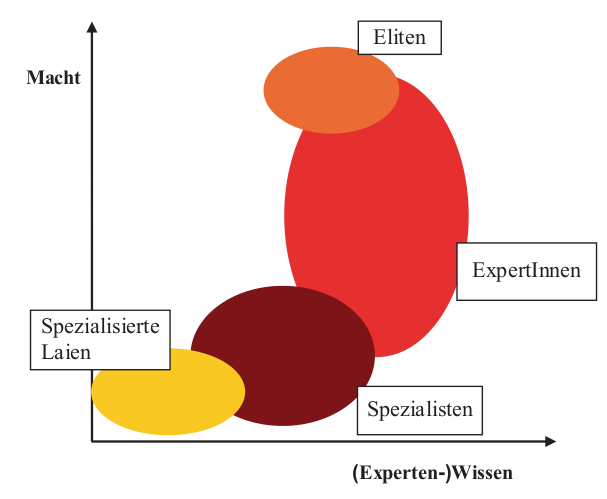
\includegraphics[width=0.8\textwidth]{Anhang/Experte}
  \quelle[o. \pno]{Littig_2008}
  \caption{Experteneinordnung}
\label{fig:experte}
\end{figure}

\glqq{}Der Experte ist -- im Gegensatz zum Spezialisten – nicht allein durch Sonderwissen in Form fachspezifischer Kompetenzen charakterisiert, sondern durch seine Fähigkeit, Verbindungen zu anderen Wissensbeständen und Wissensformen herzustellen und die Relevanz des eigenen Wissens zu reflektieren\grqq.
\footcites[][14]{Bogner_2014_Interview}[Vgl.][21 \psq]{Hitzler_1994}

Das Interessante am Expertenwissen ist nicht nur das Wissen an sich, sondern die Wirkung in der Praxis. Experten werden gefragt, weil ihre Entscheidungen und Ratschläge das Handeln anderer Akteure mitstrukturieren und -gestalten.\footcite[Vgl.][13]{Bogner_2014_Interview}

Bogner spricht davon, dass Expertenwissen \glqq seine Bedutung über [...] soziale Wirkmächtigkeit\grqq{}\footcite[][13]{Bogner_2014_Interview} erhält.
Ferner folgert er daraus die Definition:\\ \glqq Experten lassen sich als Personen verstehen, die sich -- ausgehend von einem spezifischen Praxis- oder Erfahrungswissen, das sich auf einen klar begrenzbaren Problemkreis bezieht -- die Möglichkeit geschaffen haben, mit ihren Deutungen das konkrete Handlungsfeld sinnhaft und handlungsleitend für Andere zu strukturieren.\grqq{}\footcite[][13]{Bogner_2014_Interview}

Meuser und Nagel betrachten den Experten als Konstrukt des Forschungsinteresses. Die Expertise ist also keine allgemeingültige Eigenschaft oder Fähigkeit einer Person, sondern eine Zuschreibung des Forschenden an diese, im speziellen Kontext der Forschungsfrage. \footcite[Vgl.][181]{Meuser_1994_Interview}

Zusammenfassend lässt sich also sagen, dass Experten über besonderes Wissen auf einem Gebiet verfügen und eine machtvolle Positionen innehaben können, die zwischen Spezialisten und Eliten liegt. Die Expertise muss nicht durch einen Titel oder Ähnliches verifiziert werden, sie kann auch durch jahrelange berufliche oder private Auseinandersetzung mit einem Thema erlangt werden.

Die Aufgabe des Forschers ist es demzufolge, die Experten für seine spezielle Forschungsfrage ausfindig zu machen und zu befragen.

Im Falle dieser Arbeit stammen die Experten aus dem beruflichen Umfeld des Autors und haben sich durch wichtige Positionen oder herausragende Leistungen auf dem Gebiet des Forschungsthemas hervorgetan.



\subsection{Vorstellung}
Als Experten zur Befragung wurden die \acs{IVZ} Mitarbeiter Alexander Hemmerich und Jörg Middendorf, sowie die synetics Mitarbeiter Konrad Buck und Daniel Kirsten ausgewählt.

Hemmerich und Middendorf sind seit 2011 Teil der \acs{IVZ} Belegschaft und können daher aus einiger Erfahrung schöpfen. Hemmerich ist aktuell Leiter des Rechenzentrums am Standort Köln mit den Tätigkeitsschwerpunkten Storage, Backup und Loadbalancer. Somit hat er einen guten Gesamtüberblick über die Tätigkeiten des Rechenzentrums.\\
Middendorf ist neben der Unix- und Storage Administration auch für die \acs{CMDB} des \acs{IVZ} zuständig und hat somit ein umfangreiches Wissen über Infrastruktur, Aufbau, Funktionen und Schnittstellen der \acs{CMDB}.

%Heisig ist Programmierer und IT-Consultant bei i-doit, und beschäftigt sich schwerpunktmäßig mit \acf{ITSM}, DevOps und Informationssicherheit. Außerdem hat er den \textit{i-doit-cli} Client geschrieben.\\
%Durch seine Tätigkeit hat er einen tiefen Einblick in Aufbau und Funktion einer \acs{CMDB} und kann aus den Beziehungen mit anderen Kunden von i-doit schöpfen und einschätzen, wie eine \acs{CMDB} in der Praxis verwendet wird, wie die Akzeptanz für Neuerungen ist und ob der Einsatz von Chatbots in dem jeweiligen Zusammenhang die Arbeit erleichtern könnte.\\
%Durch seine Arbeit mit dem \textit{i-doit-cli} Client kennt er sich außerdem mit der API aus und kann einschätzen, welche Funktionen, mit welchem Aufwand, automatisiert in einem Chatbot umgesetzt werden können.

Buck ist PR- und Community-Manager sowie Kommunikationsberater der synetics GmbH für das Produkt i-doit. Er hat  Publizistik und Germanistik studiert und sich als IT-Fachjournalist fortgebildet. Für synetics übernimmt er die Moderation und Kundenkommunikation, um für dauerhafte Kundenbindung zu sorgen. Durch seine Tätigkeiten hat er ein gutes Gesamtbild der Unternehmen, die eine i-doit \acs{CMDB} des Herstellers synetics einsetzen und kann den Nutzen von ChatOps für diese beurteilen. 
\footcites[Vgl.][o. \pno]{Buck_2018_Allgemein}[Vgl.][o. \pno]{Buck_2018_Referenzen}

Kirsten arbeitet seit 1998 bei der synetics GmbH und ist Produktmanager für die i-doit \acs{CMDB}. Zuvor war er als IT-Berater im Bereich Infrastruktur und Server tätig und konnte Erfahrung zu den Themen Routing/Switching, virtuelle Umgebungen und Speichernetze sammeln.
\footcite[Vgl.][o. \pno]{Kirsten_2017}

Die Experten selbst haben nicht direkt mit Chatbots zu tun, sondern sollen sie in ihrem beruflichen Kontext, auf dem sie Experten sind, also Rechenzentrumsbetrieb und \acs{CMDB}, bewerten.\\
Durch die genannten Experten werden wichtige Schlüsselfunktionen betrachtet und deren Perspektiven berücksichtigt. Auf normale \textit{Verwender} der \acs{CMDB} kann daher als Interviewpartner verzichtet werden.


\section{Ermittlung der Anforderungen an einen CMDB Chatbot}
Die Ermittlung der Anforderungen ist der erste Schritt des Anforderungsmanagements. Im Experteninterview werden darunter die ersten beiden Schritte \textit{Leitfadenerstellung} und \textit{Tonaufnahme} verstanden.

Bei der Ermittlung der Anforderungen können verschiedene Quellen, wie z. B. Stakeholder, Dokumente oder aktive Systeme genutzt werden, um Anforderungen zu detektieren und zu verfeinern.\footcite[Vgl.][21]{Pohl_2015_Requirements}

Das Interview ist eine mögliche Befragungstechnik, bei der ein Stakeholder (Interviewpartner) vom Requirements Engineer (Interviewer) vorgegebene Fragen gestellt bekommt. Die Antworten werden protokolliert. Etwaige Rückfragen können sofort im Gesprächsverlauf geklärt werden. Durch geschickt gestellte Fragen können auch unterbewusste Anforderungen ermittelt werden. Der Verlauf des Gesprächs kann individuell angepasst werden, es wird gezielt nachgefragt und auf einzelne Themen eingegangen, um das behandelte Thema möglichst komplett abzubilden.\footcite[Vgl.][28]{Pohl_2015_Requirements}

\subsection{Leitfadenerstellung}
Der Einsatz eines Leitfadens dient dazu, das Interview thematisch zu begrenzen und würdigt den Expertenstatus durch die damit verbundene Auseinandersetzung mit dem Thema. Der Leitfaden ist dabei nicht strikt zu befolgen, sondern bietet lediglich das Grundgerüst des Interviews. Reihenfolge und Tiefe der Fragen bzw. Themenkomplexe können zwischen den Interviews variieren. Die Fragen sollten dabei nicht abgelesen werden, sondern in der \glqq{}Sprache des Experten\grqq
\footcite[][449]{Meuser_1991_Interview}
gestellt werden.
\footcite[Vgl.][448\psq]{Meuser_1991_Interview}

Leitfäden in der qualitativen Forschung liegen in Art und Umfang in verschiedensten Ausprägungen vor. Je nach Forschungs- und Interviewstil reichen sie von groben Themensammlungen bis hin zu ausführlichen Leitfäden mit ausformulierten Fragen.\\
Ein Leitfaden besteht aus verschiedenen Themenblöcken, mit darin enthaltenen Hauptfragen, die sich weiter in Teilaspekte aufgliedern können. Die Hauptfragen sollten bei dem Interview auf jeden Fall zur Sprache kommen und die Teilaspekte können angesprochen werden, um die Frage zu vertiefen.
\footcite[Vgl.][27\psq]{Bogner_2014_Interview}

Der allgemeingültige Leitfaden für alle in dieser Untersuchung zu Wort kommenden Experten ist in \autoref{Leitfaden} zu finden. Er gliedert das Thema in die drei Themenkomplexe \textit{CMDB im Rechenzentrum}, \textit{Chatbots allgemein} und \textit{Chatbots zur Bedienung der CMDB}.

\subsection{Tonaufnahme}
Die Interviews mit Alexander Hemmerich und Jörg Middendorf wurden persönlich durchgeführt und mit der Audiorekorderfunktion eines Handys aufgezeichnet. Die Interviews mit Daniel Kirsten und Konrad Buck erfolgten in dem Konferenztool Cisco Webex Meeting und wurden mit dessen Aufnahmefunktion aufgezeichnet.

%Die Nachbearbeitung erfolgte mit der Software \textit{Audacity}. Sie unterstützt Features wie das Vor- und Zurückspringen und das Setzen von Markierungen.



\section{Dokumentation der Anforderungen}
Die Dokumentation der Anforderungen ist der zweite Schritt des Anforderungsmanagements. Im Experteninterview werden darunter die Schritte drei bis fünf, \textit{Transkription}, \textit{Paraphrase} und \textit{(Bildung von) Überschriften} verstanden und es ist das einzelne Interview im Fokus.

Die erarbeiteten Anforderungen werden in natürlicher Sprache oder in dafür vorgesehenen Modellen dokumentiert, wobei entsprechende Techniken zum Einsatz kommen. \footcite[Vgl.][4]{Pohl_2015_Requirements}

Die im Requirements Engineering anfallenden Tätigkeiten müssen geeignet dokumentiert werden. Dazu zählt z. B. auch die Erstellung von Interviewprotokollen. Als Dokumentation gilt jede Form der formalen Darstellung, von Beschreibung in natürlicher Sprache über strukturierten Text bis hin zu formalen Techniken wie Diagrammen. Die Dokumentationsform sollte der zugrundeliegenden Aktivität angemessen sein und diese sinnvoll wiedergeben. \footcite[Vgl.][35\psqq]{Pohl_2015_Requirements}


\subsection{Transkription}
Das Hauptaugenmerk von Experteninterviews liegt auf der Gewinnung von Wissen. Daher ist eine mühselige Notation, wie sie bei narrativen Interviews vorgenommen wird nicht nötig. Elemente wie Pausen, Betonung oder Stimmlage werden nicht interpretiert.
Eine Transkription wird in der Regel nicht für die gesamte Tonaufnahme durchgeführt, sondern kann selektiv erfolgen. Bei der Abfrage von Betriebswissen fällt die Transkription umfangreicher aus als bei Kontextwissen. \footcite[Vgl.][455\psq]{Meuser_1991_Interview}

Zur Transkription wurden die Audioaufnahmen unter Linux mit \acf{MPD} wiedergegeben und mit dem \acf{MPC} gesteuert. Dieser erlaubt die Bedienung des Backends mit Kommandozeilenbefehlen. So lassen sich globale Tastaturkürzel festlegen, um die Wiedergabe zu pausieren oder einige Sekunden zurückzuspringen und diese können genutzt werden, um die Wiedergabe zu steuern, ohne den Editor zu verlassen oder die Hände von der Tastatur zu heben.

Die Transkripte der Interviews sind in \autoref{Interview_Hemmerich}, \autoref{Interview_Middendorf}, \autoref{Interview_Kirsten} und \autoref{Interview_Buck} zu finden.


\subsection{Paraphrase}
Die Paraphrase erfolgt unter Berücksichtigung der Forschungsfrage und gibt die Aussagen der Experten chronologisch geordnet und unverfälscht wieder, wobei diese zu thematischen Verbünden zusammengefasst werden. Ob die Passage zusammenfassend oder detailliert wiedergegeben wird hängt von der Priorität des Themas und nicht zwangsläufig von der ihm gewidmeten Zeit ab.
\footcite[Vgl.][456\psq]{Meuser_1991_Interview}

In den folgenden Abschnitten werden die einzelnen Interviews paraphrasiert. Dabei werden die in \autoref{ueber} vorgesehenen Überschriften der besseren Lesbarkeit halber bereits der Passage vorangestellt.

\subsubsection{Interview Hemmerich}
\textbf{\acs{CMDB} allgemein: }Es soll zunächst das Interview mit Alexander Hemmerich betrachtet werden. Er beschreibt die \acs{CMDB} als Tool, um \glqq{}Configuration Items im Rechenzentrum, vom Kabel über Server über Ausstattung innerhalb eines Rechnerraums\grqq
\footcite[][o. \pno]{Hemm_2019}
zu verwalten und zählt auch die vermerkten Lizenzen und Supportverträge dazu.\\
Seiner Meinung nach lässt sich die Vielzahl an Komponenten \glqq{}gar nicht mehr anders handhaben\grqq
\footcite[][o. \pno]{Hemm_2019}.
Außerdem führt er an, dass die \acs{CMDB} gefordert sei, um eine ISO 27001 Zertifizierung zu erlangen.
\footcite[Vgl.][o. \pno]{Hemm_2019}

\textbf{Bestandsprüfung, Statusabfrage, Ressourcenübersicht: }Bei der täglichen Arbeit nutzt Hemmerich die \acs{CMDB} \glqq{}[u]m Gegenstände und Bestände abzufragen\grqq
\footcite[][o. \pno]{Hemm_2019}
, also beispielsweise zur Prüfung des aktuellen Kabelbestands im Lager oder um den Status eines Servers abzufragen (eingelagert, verschrottet, etc.).\\
Außerdem nutzt er die Report Funktion, um zu ermitteln welche Ressourcen ein Kunde oder eine Anwendung belegt (RAM, CPU, etc.). Dies sei einerseits bei der Abrechnung ausschlaggebend und andererseits bei der Beantragung neuer Dienstleistungen, wie \glqq{}zusätzliche[n] virtuelle[n] Maschinen\grqq
\footcite[][o. \pno]{Hemm_2019}
,nötig, um festzustellen, ob die Anforderungen durch den bestehenden Vertrag abgebildet sind oder ob eine Erweiterung erfolgen muss. \glqq{}[D]as ... [geht] ... zu unserem Vertrieb und daraus entsteht ... eine Preisinformation für den Kunden\grqq
\footcite[][o. \pno]{Hemm_2019}
.
\footcite[Vgl.][o. \pno]{Hemm_2019}

\textbf{\acs{CMDB} Schnittstellen: }Hemmerich hält die \acs{CMDB} für besonders wichtig, da sie \glqq{}das führende System ist\grqq
\footcite[][o. \pno]{Hemm_2019}
. Das Monitoring System und ein Scan System liefern Daten zu und diese werden in der CMDB \glqq{}aggregriert, um eine Gesamtsicht auf das Rechenzentrum, auf die Ausstattung und sogar auf die Standorte des Unternehmens zu bieten.\grqq
\footcite[][o. \pno]{Hemm_2019}
.\\
Außerdem ergänzt er, dass neben Configuration Items des Rechenzentrums auch Gebäude, Büros und Mitarbeiter in der \acs{CMDB} vermerkt sind.
\footcite[Vgl.][o. \pno]{Hemm_2019}

\textbf{Chatbots allgemein: }Als Chatbots betrachtet Hemmerich Bots, \glqq{}mit denen man kommunizieren kann\grqq
\footcite[][o. \pno]{Hemm_2019}
und die auf Anfrage \glqq{}Informationen liefern\grqq
\footcite[][o. \pno]{Hemm_2019}
oder \glqq{}Aktion[en] ausführen\grqq
\footcite[][o. \pno]{Hemm_2019}
. Persönlich hat er noch keine Erfahrungen mit Chatbots oder ChatOps gemacht, er blickt jedoch gespannt auf deren großes Einsatzspektrum.
\footcite[Vgl.][o. \pno]{Hemm_2019}

\textbf{Chatbots zur Automatisierung: }Als Ersatz für menschliche Arbeitskräfte betrachtet Hemmerich Chatbots nicht, sondern vielmehr als Unterstützung bei der täglichen Arbeit. \glqq{}Ein Chatbot könnte einfache Tätigkeiten übernehmen und zur Automatisierung des täglichen Rechenzentrumsbetriebs beitragen.\grqq
\footcite[][o. \pno]{Hemm_2019}
Aus seiner Sicht können dadurch alltägliche Arbeitsschritte vereinfacht werden.
\footcite[Vgl.][o. \pno]{Hemm_2019}

\textbf{Suchfunktion, Nächste freie IP, Serverplanung, Schnittstellenanbindung: }Als mögliche Funktionen für einen Chatbot, der die \acs{CMDB} bedient kann Hemmerich sich die Suche nach Objekten und die Anzeige der nächsten freien IP-Adresse in einem bestimmten Netz vorstellen.
Dabei hat er einen Workflow vor Augen, bei dem ein Server über den Bot geplant und mit einem Namen versehen wird. Daraufhin soll für diesen eine freie IP-Adresse in einem bestimmten Netz gesucht und reserviert werden.\\
Als sinnvolle Ergänzung würde er hier begrüßen, dass in diesem Workflow direkt die virtuelle Maschine bereitgestellt, die Konfiguration per Puppet vorgenommen und die Netzkonfiguration hergestellt wird. Davon verspricht er sich eine Vermeidung von Inkonsistenzen zwischen CMDB und Realität. 
\footcite[Vgl.][o. \pno]{Hemm_2019}\\
Dies übersteigt den \acs{CMDB}-Fokus, kann jedoch im Ausblick und in der Möglichkeit einer Anbindung von weiteren Tools und Schnittstellen berücksichtigt werden.

\textbf{Vermeidung Fehlbedienung, Berechtigungskonzept, Nachvollziehbarkeit: }Die Integrität der \acs{CMDB} ist für Hemmerich ein hohes Gut und eine versehentliche Löschung oder Manipulation von Daten durch \glqq{}Fehlfunktion oder Fehlbedienung [des] Bots\grqq
\footcite[][o. \pno]{Hemm_2019}
sollte vermieden werden. Bei der Entwicklung sollte darauf geachtet werden, die Betriebssicherheit zu gewährleisten.\\
Außerdem legt Hemmerich Wert darauf, dass nur ein bestimmter Personenkreis berechtigt ist, Änderungen oder Löschungen vorzunehmen und es soll nachvollziehbar sein, wer Änderungen vorgenommen hat.
\footcite[Vgl.][o. \pno]{Hemm_2019}

\textbf{Akzeptanz, Webinterface Eingaben: }Probleme erwartet Hemmerich bei der Einführung eines \acs{CMDB} Chatbots nicht, er könnte sich jedoch vorstellen, dass ältere Kollegen etwas Zeit brauchen, um sich daran zu gewöhnen und lieber weiterhin die Eingaben über das Webinterface vornehmen. 
Da es sich aber größtenteils um junge, motivierte Menschen handelt, \glqq{}die auch in der Freizeit viel mit neuen Technologien arbeiten\grqq
\footcite[][o. \pno]{Hemm_2019}
, erwartet Hemmerich, dass ein \acs{CMDB} Chatbot \glqq{}in dem Bereich sehr großen Anklang finden wird\grqq
\footcite[][o. \pno]{Hemm_2019},
\footcite[Vgl.][o. \pno]{Hemm_2019}

\textbf{Transparenz, Arbeitsüberwachung: }Die ChatOps-inherente Transparenz befürwortet Hemmerich grundsätzlich. Er gibt jedoch zu bedenken, dass man darin eine Form von Arbeitsüberwachung sehen kann. In einem transparenten Chat Raum sei es denkbar, dass man nachvollziehen kann, woran und wie intensiv andere Kollegen arbeiten, deshalb solle man diesbezüglich Rücksprache mit dem Betriebsrat halten.\\
Seitens der Kollegen rechnet er mit Zustimmung und Offenheit für diese Arbeitsweise. 
\footcite[Vgl.][o. \pno]{Hemm_2019}

\textbf{Framework Python, Weiterentwicklung: }Bei der Wahl des Bot-Frameworks legt Hemmerich Wert auf die Wartbarkeit und Möglichkeit der Weiterentwicklung. Aufgrund des fundierten Python Know-Hows im Rechenzentrum würde er einen Bot in dieser Sprache bevorzugen. Er empfiehlt, \glqq{}Entwicklungen in den Sprachen zu betreiben, wo das Know-How da ist und auch in Zukunft da sein wird. Denn es gibt nichts Schlimmeres als eine Anwendung, die ein Praktikant oder Azubi entwickelt hat in einer Sprache, mit der sich hier keiner auskennt und die nach seinem Weggang eben nicht mehr wartbar ist.\grqq
\footcites[][o. \pno]{Hemm_2019}[Vgl.][o. \pno]{Hemm_2019}

\textbf{Charakter, Avatar: }Bei der Modellierung der Persönlichkeit des \acs{CMDB} Chatbots verweist Hemmerich auf die Professionalität des Rechenzentrumsbetriebs und schlägt einen dementsprechenden Charakter vor. Da das Unternehmen im Medienbereich tätig ist, könnte er sich Maus oder Elefant aus der Sendung mit der Maus als Avatar vorstellen. Da im Alltag eine humorvolle Stimmung herrscht, würde er einen solchen Charakterzug befürworten.  
\footcite[Vgl.][o. \pno]{Hemm_2019}

\textbf{Betriebssicherheit: }\glqq{}[I]m Hinblick auf die Betriebssicherheit\grqq
\footcite[][o. \pno]{Hemm_2019}
zieht Hemmerich einen regelbasierten Chatbot einem KI-gestützten vor, da das Regelwerk klar definiert werden kann und keine ungeplanten oder unbeabsichtigten Aktionen ausgeführt werden, die im schlimmsten Fall zu \glqq{}einer Katastrophe oder Störung\grqq 
\footcite[][o. \pno]{Hemm_2019}
 führen können. 
\footcite[Vgl.][o. \pno]{Hemm_2019}

\textbf{Potential: }Auch für andere Tätigkeiten des Rechenzentrums sieht Hemmerich \glqq{}großes Potential\grqq
\footcite[][o. \pno]{Hemm_2019}
 in der Verwendung von ChatOps.
 Er warnt davor, sich vor einer solchen Technologie zu fürchten und sie als Bedrohung des eigenen Arbeitsplatzes zu sehen. Stattdessen sei sie eine \glqq{}sinnvolle Ergänzung der täglichen Arbeit\grqq
\footcite[][o. \pno]{Hemm_2019}
. Auch für andere Unternehmen kann er sich eine ChatOps Lösung vorstellen. \glqq{}Jeder der eine CMDB einsetzt, kann von so etwas nur profitieren.\grqq
\footcites[][o. \pno]{Hemm_2019}[Vgl.][o. \pno]{Hemm_2019}



\subsubsection{Interview Middendorf}
\textbf{CMDB allgemein: }Als nächstes soll das Interview mit Jörg Middendorf betrachtet werden. Unter einer \acs{CMDB} versteht er eine Datenbank, in der \glqq{}alle Gerätschaften eines Unternehmens dokumentiert sind und in Relation gesetzt werden\grqq.
\footcite[][o. \pno]{Midd_2019}
.
Z. B. werden \glqq{}Server, Lizenzen und Aufstellungsorte\grqq
\footcite[][o. \pno]{Midd_2019}
 dokumentiert, um sie für Supportfälle oder Planungstätigkeiten zu nutzen.
\footcite[Vgl.][o. \pno]{Midd_2019}

\textbf{Suchfunktion, Standortabfrage, Standortreport: }Bei der täglichen Arbeit nutzt Middendorf die \acs{CMDB} vor Allem zur \glqq{}Dokumentation neu erstellter Maschinen\grqq
\footcite[][o. \pno]{Midd_2019}
 und um Objekte wie Server zu suchen und deren Standort zu überprüfen. Außerdem nutzt er die Reporting Funktion zur Unterstützung bei Planungen, z. B. um festzustellen, \glqq{}wie viele Server an einem Standort ... sind\grqq
\footcite[][o. \pno]{Midd_2019}
. Durch ein aktuelles \glqq{}Projekt, bei dem Rechenzentren umgezogen werden\grqq
\footcite[][o. \pno]{Midd_2019}
 wird diese Funktionalität häufig benötigt. Abseits davon nutzt er die \acs{CMDB} um IP-Netze zu dokumentieren und neue Adressen zu vergeben, bzw. nachzuprüfen, wofür bestehende genutzt werden.
\footcite[Vgl.][o. \pno]{Midd_2019}

\textbf{CMDB Schnittstellen: }Besonders wichtig findet Middendorf die Schnittstellen der \acs{CMDB}. Es gibt einerseits die Möglichkeit, aus dem Monitoring Daten abzufragen und andererseits die Möglichkeit, in \glqq{}der CMDB geplante Daten ins Monitoring zu transferieren\grqq
\footcite[][o. \pno]{Midd_2019}
.
Außerdem findet er die Reporting-Funktion für die tägliche Arbeit sehr wichtig.
\footcite[Vgl.][o. \pno]{Midd_2019}

\textbf{ChatOps allgemein: }ChatOps versteht Middendorf im DevOps-Gedanken, also als Zusammenarbeit von Entwicklern und Administratoren.
Mit Chatbots hatte er vor Allem schon bei Supportanbietern zu tun, die diese einsetzen, um \glqq{}Anliegen aufzunehmen und zu klassifizieren\grqq
\footcite[][o. \pno]{Midd_2019}
.
Auch mit Sprachassistenten, wie Siri oder Alexa hatte er bereits zu tun.
\footcite[Vgl.][o. \pno]{Midd_2019}

\textbf{Softwarestand, IP-Adresse, Automatisierung: }Im Rechenzentrumsbereich sieht Middendorf für Chatbots vor allem Potential, Standardaufgaben zu übernehmen. Dazu zählt er die Suche nach dem Standort von Geräten und die Ermittlung von Softwareständen und IP-Adressen. Für diese Aufgaben werden bisher die RZ-Mitarbeiter persönlich oder per E-Mail gefragt. Von einer Automatisierung per Chatbot verspricht er sich für die Mitarbeiter eine Konzentration auf die eigentlichen Aufgaben des RZ-Betriebs.
\footcite[Vgl.][o. \pno]{Midd_2019}

\textbf{Mobilität, IP-Adresse, Netzinformationen, Ressourcen: }Als Vorteil eines Chatbots zur Bedienung der \acs{CMDB} sieht Middendorf vor Allem die Mobilität. Als konkretes Beispiel könne er sich hier vorstellen, bereits auf dem Weg zum Rechenzentrum nach einem Server zu suchen, um herausfinden, in welchem Rack und an welcher Position sich dieser befindet. Außerdem könne er vor Ort prüfen, welche Software der Maschine zugewiesen ist, welche IP sie hat, welchem Subnetz und VLAN sie angehört und wie viel Festplattenplatz und RAM belegt sind.
Außerdem ergänzt er, dass die Abfrage per Webinterface auf Mobilgeräten möglicherweise gar nicht möglich sei.
\footcite[Vgl.][o. \pno]{Midd_2019}

\textbf{Servereinbau, Serverausbau: }Als Möglichkeit zur Arbeitsvereinfachung sieht Middendorf einen \acs{CMDB} Chatbot auch beim Einbau von neuer Hardware im Rechenzentrum. So könne er direkt den Einbauort vermerken, den Server benennen und ihm eine IP-Adresse zuweisen. Beim Ausbau eines Geräts könne er hingegen den Status des Geräts auf \textit{außer Betrieb} oder \textit{verschrottet} setzen.
\footcite[Vgl.][o. \pno]{Midd_2019}

\textbf{Berechtigungskonzept, API Einsatz: }Nach Middendorfs Ansicht sollte nur ein bestimmter Personenkreis Zugriff auf die \acs{CMDB} Features haben. Dies gelte vor Allem für die schreibenden Funktionen, für die Lesenden sei eine andere Regelung denkbar (z. B. Öffnung der Suche für alle).
Als weitere Anfoderung gibt er vor, die \acsp{API} oder Command Line Tools des \acs{CMDB} Herstellers zu nutzen und nicht direkt auf die Datenbank zuzugreifen.
\footcite[Vgl.][o. \pno]{Midd_2019}

\textbf{Nachvollziehbarkeit: }Middendorf ergänzt weiterhin, dass nachvollziehbar sein sollte, wer welche Änderung vorgenommen hat. Dies könne beispielsweise im Chatverlauf oder in einem Log File festgehalten werden und solle dauerhaft abrufbar sein. Im Idealfall werde diese Information direkt bei der Manipulation eines \acs{CI}s als Kommentar vermerkt.
\footcite[Vgl.][o. \pno]{Midd_2019}

\textbf{Arbeitsüberwachung: }Mit Problemen beim Einsatz eines \acs{CMDB} Chatbots rechnet Middendorf grundsätzlich nicht, er gibt jedoch zu bedenken, dass eine Chat Software, die außerhalb eines Unternehmens gehostet wird und Unternehmensinterna darin kommuniziert werden, besondere Regularien erfüllen müsse. Die Transparenz, die mit ChatOps einhergeht, sieht Middendorf als Vorteil. Man könne direkt mitverfolgen, was sich in der Umgebung ändert oder sich nach Abwesenheit einen Überblick über die erfolgten Änderungen verschaffen. Allerdings solle diese Übersicht nicht zur Auswertung der Arbeitsleistung herangezogen werden.
\footcite[Vgl.][o. \pno]{Midd_2019}

\textbf{Framework: }Bei der Wahl des Bot-Frameworks sieht Middendorf Errbot in Betrachtung der Weiterentwicklung als klaren Favoriten, da im Rechenzentrum bereits großes Python Know-How vorhanden und die Sprache auch für Laien recht leicht lesbar ist.
\footcite[Vgl.][o. \pno]{Midd_2019}

\textbf{Charakter: }Als Persönlichkeit für einen Chatbot kann sich Middendorf keine konkrete Figur oder Person vorstellen. Er würde jedoch einen humorvollen Charakter bevorzugen. Es müsse aber darauf geachtet werden, dass die Aussagen des Bots nicht verletzend wirken. Bei mehrfachen Anfragen nach dem gleichen Inhalt oder Falscheingaben könne durchaus eine freche Antwort folgen. 
\footcite[Vgl.][o. \pno]{Midd_2019}

\textbf{Ansatz, Hilfe: }Bei der Wahl der Art des Chatbots spricht sich Middendorf klar für einen regelbasierten Ansatz aus. Der Bot solle nur genau das machen, was angefordert ist und nichts, das er durch künstliche Intelligenz dazu gelernt hat. Eine Interpretation solle nicht erfolgen, das Ergebnis könne dann zu stark von der Erwartung abweichen. Ein KI-gestützter Chatbot sei deshalb höchstens für andere Anwendungen, wie die Begrüßung neuer Mitarbeiter oder die Beantwortung der FAQ zu bevorzugen, nicht aber für Rechenzentrumstätigkeiten.\\
Da die RZ Mitarbeiter täglich auf Kommandozeilenebene arbeiten geht Middendorf davon aus, dass sie mit den Befehlen des Bots schnell zurecht kommen. Außerdem müsse dieser über eine Hilfe Funktion verfügen, welche die gültigen Kommandos mit Beispielen ausgibt.  Eine Einführungsveranstaltung solle vor Inbetriebnahme des Bots erfolgen.
\footcite[Vgl.][o. \pno]{Midd_2019}

\textbf{Nachfrage, Herstellerkonsolidierung: }Bei kritischen Aktionen hält Middendorf eine zusätzliche Abfrage für sinnvoll. Außerdem sei es bisher der Fall, dass der gleiche Hersteller unter unteschiedlichen Namen im System vermerkt ist (z. B. HP, Hewlett-Packard). Daher sei es sinnvoll, bei der Eintragung neuer Hardware, die bestehenden Hersteller zu berücksichtigen und bei Ähnlichkeit vorzuschlagen, um Dopplungen zu vermeiden. Dies solle interaktiv erfolgen.
\footcite[Vgl.][o. \pno]{Midd_2019}

\textbf{Potential: }Für andere Rechenzentrumstätigkeiten sieht Middendorf ebenfalls Potential. Alle Dienste mit einer API seien zur Automatisierung gut geeignet. Er könne sich z. B. die Provisionierung von virtuellen Maschinen, die Anbindung an Puppet und die Bearbeitung von DNS Einträgen vorstellen. Auch für andere Unternehmen hält er ChatOps für sinnvoll. Vor Allem die Knappheit an qualifiziertem Personal spreche für mehr Automatisierung und ein Chatbot sei dafür eine sinnvolle Möglichkeit, da er bei der täglichen Arbeit die Komplexität von Workflows reduziert.
\footcite[Vgl.][o. \pno]{Midd_2019}



\subsubsection{Interview Kirsten}
\textbf{CMDB allgemein: }Als nächstes soll das Interview mit Daniel Kirsten betrachtet werden. Er betrachtet in seiner Funktion als Produktmanager die \acs{CMDB} streng nach \acs{ITIL} und versteht darunter die zentrale Erfassung von IT-Infrastruktur Elementen und deren Konfiguration. Das Verständnis unterscheide sich dabei stark und die gespeicherten Daten reichten von Asset Management Informationen bis hin zu technischen Konfigurationen. Außerdem spreche man nach \acs{ITIL} nicht mehr von einer \acs{CMDB}, sondern eher von einem \acf{CMS}, welches eine Vereinigung mehrerer \acsp{CMDB} darstellt. Der Großteil der Anwender betrachte die \acs{CMDB} als Datenbank, die \glqq{}alle Komponenten einer IT-Infrastruktur vereint, dokumentiert und im Idealfall mindestens die technischen Grundkonfigurationen dieser Elemente aufnimmt.\grqq 
\footcites[][o. \pno]{Kirsten_2019}[Vgl.][o. \pno]{Kirsten_2019}

\textbf{Interner Einsatz: }Bei der täglichen Arbeit nutzt Kirsten selbst die i-doit \acs{CMDB}, um die internen technischen Komponenten zu dokumentieren. Sie diene als Nachschlagwerk und werde manuell, ohne Zuhilfenahme automatisierter Prozesse befüllt. Neben den internen Komponenten seien auch noch Cloud Ressourcen dort dokumentiert. 
\footcite[Vgl.][o. \pno]{Kirsten_2019}

\textbf{IP-Adressen, Passwörter, Cloud: }Die Erfassung von IP-Adressen und Passwörtern in der \acs{CMDB} findet Kirsten besonders wichtig. Da vermehrt Cloud Lösungen eingesetzt werden, sei es zudem wichtig Zugang und verknüpfte Dienste zu diesen Ressourcen zu dokumentieren.
\footcite[Vgl.][o. \pno]{Kirsten_2019}

\textbf{ChatOps, Chatbots, Output: }Mit ChatOps hatte Kirsten noch keine Berührungspunkte, im Grunde verstehe er es aber als DevOps Prozess, der durch Chatbots unterstützt wird.  Beim Thema Chatbots kann er aus einiger Erfahrung schöpfen, da er fast zehn Jahre lang TCL Skripte für Eggdrop Bots programmierte. Einen Chatbot definiert er als Instanz, die User Input entgegennimmt, verschiedene Datenquellen nutzt und einen menschenlesbaren Output liefert.
\footcite[Vgl.][o. \pno]{Kirsten_2019}

\textbf{Vorteile Chatbots: }Als Vorteil von Chatbots sieht Kirsten den schnellen Abruf von Informationen. Damit spare man sich z. B. das Öffnen des Browsers und die Anmeldung. Er warnt jedoch auch davor, zu viele Informationen von einem Chatbot ausgeben zu lassen. Für die gängigsten Funktionen einer \acs{CMDB} kann Kirsten sich einen Chatbot gut vorstellen. 
\footcite[Vgl.][o. \pno]{Kirsten_2019}

\textbf{IP-Adressen, Standortdaten, Kontaktpersonen, Suche, Logbuch: }Da der Output von Chatbots auf Text limitiert ist, empfiehlt Kirsten, die Prozesse eines Chatbots nicht zu komplex zu gestalten. Als konkrete Anwendungsfälle eines \acs{CMDB} Chatbots könne er sich die Abfrage von IP-Adressen, Standortdaten oder Kontaktpersonen vorstellen. Außerdem sei eine Suche sinnvoll, wenn man den kompletten Objektnamen nicht weiß. Zudem könne er sich vorstellen, freie IP-Adressen zu reservieren oder als Administrator Änderungen am Logbuch zu erfassen. Vor Allem die Ausgabe von Informationen hält Kirsten für leicht umsetzbar, die Eingabe stehe eher im Hintergrund, da die Normalisierung fehleranfällig ist.
\footcite[Vgl.][o. \pno]{Kirsten_2019}

\textbf{Rechtesystem, Plattform-Agnostik: }Ein \acs{CMDB} Chatbot soll laut Kirsten ein Rechtesystem abbilden, das nur den Nutzern Informationen darstellt, die berechtigt sind, diese zu sehen. Er sehe sonst ein Missbrauchspotential. Außerdem rät er dazu, einen Chatbot nur im internen Netz zu betreiben, um die \acs{CMDB} nicht für das Internet zugänglich zu machen. Weiterhin rät er dazu, den Chatbot möglichst plattform-agnostisch zu gestalten, also die Möglichkeit zu bieten, \glqq{}verschiedene Chatsysteme daran anzubinden\grqq
\footcite[][o. \pno]{Kirsten_2019}
. Als Standard sehe er jedoch aktuell Slack.
\footcite[Vgl.][o. \pno]{Kirsten_2019}

\textbf{Akzeptanz, Feedback: }Mit Problemen bei der Akzeptanz eines \acs{CMDB} Chatbots rechnet Kirsten nicht. Es müsse einer die Funktionen in einem öffentlichen Raum nutzen, damit andere das Potential erkennen und es ihm gleich tun. So könne Viralität entstehen. Man erhalte als Entwickler jedoch kaum Feedack. Wenn der Bot nicht angenommen wird, spiegele es sich lediglich darin, dass er nicht genutzt wird. Generell ist Kirsten jedoch zuversichtlich bezüglich der Akzeptanz eines \acs{CMDB} Chatbots.
\footcite[Vgl.][o. \pno]{Kirsten_2019}

\textbf{Programmiersprache: }Wegen der großen Verbreitung, der Mächtigkeit und dem langen Bestehen, empfiehlt Kirsten als Programmiersprache Python. Bei neueren Technologien wie Ruby oder Coffeescript rate er eher zur Vorsicht. 
\footcite[Vgl.][o. \pno]{Kirsten_2019}

\textbf{Persönlichkeit, Avatar: }Dem CMDB Chatbot eine Persönlichkeit zu verleihen hält Kirsten nicht für notwendig. Da vorwiegend Techniker damit arbeiten sollen, seien Formalitäten wie Begrüßungen überflüssig. Als Avatar könne er sich jedoch einen Roboter vorstellen. 
\footcite[Vgl.][o. \pno]{Kirsten_2019}

\textbf{Ansatz: }Kirsten spricht sich für einen regelbasierten Chatbot aus, ein KI-gestützter Bot sei eher schwierig und führe zu Frustationen beim Anlernen. Er empfiehlt die Konzentration auf \glqq{}kleine, regelbasierte Aufgaben\grqq
\footcites[][o. \pno]{Kirsten_2019}[Vgl.][o. \pno]{Kirsten_2019}

\textbf{Potential: }Für andere Unternehmen sieht Kirsten großes Potential für die Verwendung eines \acs{CMDB} Chatbots. Vor Allem durch die Verwendung von Slack und Whatsapp seien die Anwender mit dem Medium vertraut und können damit professionell umgehen. Schnittstellen dazu zu haben, halte er daher für sinnvoll.
\footcite[Vgl.][o. \pno]{Kirsten_2019}

\textbf{Reaktivität: }Ergänzend warnt Kirsten davor, Funktionen zu nutzen, die automatisch Inhalte darstellen. Dadurch gingen Informationen verloren und niemand reagiere darauf. Daher solle ein \acs{CMDB} Chatbot rein reaktiv arbeiten. 
\footcite[Vgl.][o. \pno]{Kirsten_2019}



\subsubsection{Interview Buck}
\textbf{\acs{CMDB} allgemein: }Als Letztes soll das Interview mit Konrad Buck betrachtet werden. Unter einer \acs{CMDB} versteht er eine Datenbank, die dynamisch alle für den IT-Betrieb notwendigen Items aufnimmt und verwaltet, um einen effektiven Betrieb zu gewährleisten, Prozesse zu planen und Changes durchzuführen.
\footcite[Vgl.][o. \pno]{Buck_2019}

\textbf{CMDB Funktionen: }Besonders wichtig findet Buck dabei die UI, also die grafische Darstellung von Netzwerken oder Räumen mit der Möglichkeit in einzelne Bereiche hereinzuzoomen. Heutzutage seien alle an Videos und \glqq{}einfache bildliche Darstellung[en]\grqq
\footcite[][o. \pno]{Buck_2019}
 gewöhnt, weshalb Listenanzeigen unpassend sind. Außerdem müsse die Benutzerführung gut sein und es solle die Möglichkeit bestehen, Wartungspläne, Notfallpläne, Arbeitsabläufe und eine Wissensdatenbank zu organisieren. Schnittstellen solle eine \acs{CMDB} auch haben, um z. B. Ticketing und Inventarisierung anzubinden und einen Gesamtüberblick zu erlangen. 
\footcite[Vgl.][o. \pno]{Buck_2019}

\textbf{Chatbots, ChatOps: }Unter einem Chatbot versteht Buck ein Programm, das zur Automatisierung genutzt wird. Damit sei es möglich, Tätigkeiten wie die Kommunikation mit dem Herstellersupport oder Service-Management abzulösen und vorgefasste Antworten auf häufige Fragen zu entgegnen. Mit ChatOps hat Buck bisher noch keine Erfahrungen.
\footcite[Vgl.][o. \pno]{Buck_2019}

\textbf{Kontakt Chatbots: }Persönlich hatte Buck bisher nur in Warteschleifen von Hotlines Kontakt mit Chatbots, die das Anliegen erfassen, kategorisieren und an einen echten Mitarbeiter weiterleiten.
\footcite[Vgl.][o. \pno]{Buck_2019}

\textbf{Standardanfragen, Vorhersage, Sprachassistenten: }Laut Buck könnte ein \acs{CMDB} Chatbot sämtliche Standardanfragen, die ein Admin sonst übernimmt bearbeiten. Der Bot müsste dafür an eine Wissensdatenbank mit entsprechenden Fragen angebunden werden.
Als weiteres Feature betrachtet Buck die Vorhersage von Zuständen, also z. B. der Resssourcenbelegung von Servern, um Aktionen zu planen. Außerdem sehe er Sprachassistenten als mögliches Interface, da diese in der Lage seien Emotionalität in der Stimme zu erkennen. In der Verbindung mit dem Profil des Nutzers könne so die Intention besser verstanden werden. Er sieht in einem \acs{CMDB} Chatbot die Chance, Workflows zu vereinfachen, eine Zeitersparnis zu erzielen und die Akzeptanz bei Endanwendern zu verbessern. 
\footcite[Vgl.][o. \pno]{Buck_2019}

\textbf{Vertrauen, Gemütszustand: }Buck vermutet, dass die Benutzer der \acs{CMDB} anderen Menschen mehr vertrauen als einer Maschine, was zu einer Skepsis bei der Verwendung von Chatbots führen könnte. Beim Thema Sicherheit hingegen hat er keine Bedenken, es handele sich lediglich um eine Verschiebung \glqq{}der Schnittstelle zwischen Mensch und Maschine\grqq
\footcite[][o. \pno]{Buck_2019}
. Er verspricht sich sogar einen Gewinn an Sicherheit, da ein sprachbasierter Chatbots anhand der Stimme Müdigkeit oder Desinteresse erkennen und eine Fehlbedienung vermeiden könne. 
\footcite[Vgl.][o. \pno]{Buck_2019}

\textbf{Akzeptanz: }Buck rechnet damit, dass Chatbots einen schweren Einstieg haben werden, da sie oftmals nur aus Telefonwarteschleifen bekannt sind. Davon müssten sich professionelle Chatbots abheben. 
\footcite[Vgl.][o. \pno]{Buck_2019}

\textbf{Avatar, Persönlichkeit: }Als Avatar für einen \acs{CMDB} Chatbot kann Buck sich \textit{Dschinni} vorstellen und als Persönlichkeit eine Mischung aus Professionalität und Lockerheit. Ein Chatbot müsse die notwendige Professionalität ausstrahlen, damit ein Administrator seine Arbeit erledigen kann.
\footcite[Vgl.][o. \pno]{Buck_2019}

\textbf{Ansatz: }Bei der Wahl des Chatbots spricht sich Buck klar für eine KI-gestützte Variante aus. Diese sei insbesondere bei der Verwendung von Stimmerkennung vorteilhaft. Allerdings merkt er auch an, dass die KI-Unterstützung recht kostspielig sein kann und deshalb für kleinere Unternehmen eher nicht in Frage kommt. Die Gefahr von Fehlinterpretationen durch KI-Systeme schätzt Buck eher gering ein. Er setze voraus, dass die Anbieter solcher Lösungen dies im Griff haben.
\footcite[Vgl.][o. \pno]{Buck_2019}

\textbf{Potential: }Auch für andere Unternehmen sieht Buck Potential für die Verwendung eines \acs{CMDB} Chatbots. Vor Allem die Neuheit des Themas und die mögliche Arbeitserleichterung sei dabei ausschlaggebend. Über das Thema KI werde häufig gesprochen, allerdings gebe es kaum konkrete Anwendungen dafür. Dann müsse aber auch eine entsprechende Plausibilitätsprüfung durchgeführt und Sicherheit gewährleistet werden.
\footcite[Vgl.][o. \pno]{Buck_2019}



\subsection{(Bildung von) Überschriften} \label{ueber}
Die paraphrasierten Abschnitte werden möglichst textnah mit einer oder mehreren Überschriften versehen, je nach dem, wie viele Themen angesprochen werden. Dabei ist darauf zu achten, dass das Expertenwissen im Fokus steht, der Experte als Person ist nicht relevant.\footcite[Vgl.][458\psq]{Meuser_1991_Interview}

Die Anforderungen aus den paraphrasierten Textpassagen werden im Folgenden in \autoref{tab:expmidd}, \autoref{tab:exphemm}, \autoref{tab:expkirs} und \autoref{tab:expbuck} pro Interview mit Überschriften versehen und in der Reihenfolge der Nennung tabellarisch dargestellt. Außerdem werden sie in funktionale Anforderungen und Qualitätsanforderungen eingeteilt.

Funktionale Anforderungen legen fest, welche Funktionalität ein System bieten soll. Sie können weiter in Funktions-, Verhaltens- und Strukturanforderungen unterteilt werden. In den Anforderungen werden diese mit einem \textit{F} im Bezeichner vermerkt.
\footcite[Vgl.][8]{Pohl_2015_Requirements}

Qualitätsanforderungen beschreiben die Qualitäten, die ein System erfüllen muss und beeinflussen die Systemarchitektur. Typische Qualitätsanforderungen sind z. B. Performance, Verfügbarkeit, Skalierbarkeit oder Portabilität. In den Anforderungen werden diese mit einem \textit{Q} im Bezeichner vermerkt.
\footcite[Vgl.][9]{Pohl_2015_Requirements}

Dabei werden die laut Pohl und Rupp vorgesehenen Spalten Autor und Quelle ausgelassen und nur Identifikator und Name aufgeführt, da sich die Anforderungen auf das jeweilige Experteninterview beziehen und die Quelle das Interviewprotokoll und der Autor der Interviewpartner ist.\footcite[Vgl.][126]{Pohl_2015_Requirements}

\begin{table}[H]
\centering
\begin{tabularx}{1\textwidth}{l|l|X}
  Bezeichner & Name & Anforderung \\\hline
  1-1-F  & Bestandsprüfung          & Bestand von Gegenständen im Lager (z. B. Kabel) soll geprüft werden.\\
  1-2-F  & Statusabfrage            & Der Status von Servern (eingelagert, verschrottet) soll abgefragt werden.\\
  1-3-F  & Ressourcenübersicht      & Es soll ein Report über die Ressourcen eines Kunden / einer Anwendung möglich sein.\\
  1-4-F  & Suchfunktion             & Es soll eine Suche nach Objekten möglich sein.\\
  1-5-F  & Nächste freie IP         & Es soll die nächste freie IP in einem Netz abgefragt werden können.\\
  1-6-F  & Serverplanung            & Ein neuer Server soll mit Name und IP angelegt werden können.\\
  1-7-Q  & Schnittstellenanbindung  & Bei der Entwicklung sollen zukünftige Schnittstellen zu Puppet und vCenter berücksichtigt werden.\\
  1-8-Q  & Vermeidung Fehlbedienung & Versehentliche Löschung soll vermieden werden.\\
  1-9-Q  & Berechtigungskonzept     & Nur ein bestimmter Personenkreis soll Änderungen durchführen dürfen.\\
  1-10-Q & Nachvollziehbarkeit      & Es soll nachvollziehbar sein, wer Änderungen vorgenommen hat.\\
  1-11-Q & Webinterface Eingaben    & Eingaben über das Webinterface sollen weiterhin möglich sein.\\
  1-12-Q & Arbeitsüberwachung       & Eine Auswertung der Leistung Einzelner soll nicht erfolgen. \\
  1-13-Q & Framework Python         & Es soll ein Bot-Framework in der Sprache Python gewählt werden.\\
  1-14-Q & Charakter                & Der Charakter soll Professionalität ausdrücken, aber humorvoll sein.\\
  1-15-Q & Avatar                   & Als Avatar soll Maus oder Elefant gewählt werden.\\
  1-16-Q & Betriebssicherheit       & Es soll ein regelbasierter Bot gewählt werden.\\
\end{tabularx}
\\\eigen
\caption{Anforderungen Experteninterview Hemmerich}
\label{tab:exphemm}
\end{table}

\begin{table}[H]
\centering
\begin{tabularx}{1\textwidth}{l|l|X}
  Bezeichner & Name                 & Anforderung \\\hline
  2-1-F  & Suchfunktion             & Eine Suche nach Objekten soll möglich sein. \\
  2-2-F  & Standortabfrage          & Es soll der Standort von Objekten abrufbar sein. \\
  2-3-F  & Standortreport           & Die Anzahl der Server an einem Standort soll abgefragt werden. \\
  2-4-F  & Softwarestand            & Der Softwarestand für ein Gerät soll ausgegeben werden. \\
  2-5-F  & IP-Adresse               & Die IP-Adresse eines Geräts soll ausgegeben werden. \\
  2-6-F  & Netzinformationen        & VLAN und Subnetz eines Geräts sollen ausgegeben werden. \\
  2-7-F  & Ressourcen               & HDD und RAM Belegung eines Geräts sollen angezeigt werden. \\
  2-8-F  & Servereinbau             & Beim Einbau eines Servers soll dieser mit Name, IP und Ort dokumentiert werden. \\
  2-9-F  & Serverausbau             & Beim Ausbau eines Servers soll dieser auf \textit{außer Betrieb} oder \textit{verschrottet} gesetzt werden. \\
  2-10-Q & Berechtigungskonzept     & Nur ein bestimmter Personenkreis soll Zugriff auf die schreibenden Funktionen haben. \\
  2-11-Q & API Einsatz              & Es soll per API oder Client zugegriffen werden, kein direkter Datenbank-Zugriff.\\
  2-12-Q & Nachvollziehbarkeit      & Es soll nachvollziehbar sein, wer Änderungen vorgenommen hat. \\
  2-13-Q & Arbeitsüberwachung      & Die Arbeitsleistung soll nicht ausgewertet werden. \\
  2-14-Q & Framework                & ErrBot soll als Bot Framework zum Einsatz kommen. \\
  2-15-Q & Charakter                & Der Charakter des Bots soll humorvoll sein. \\
  2-16-Q & Ansatz                   & Der Chatbot soll regelbasiert sein. \\
  2-17-Q & Hilfe                    & Der Bot soll über eine Hilfe Funktion mit Beispielen verfügen. \\
  2-18-Q & Nachfrage                & Bei kritischen Aktionen soll eine zusätzliche Abfrage zur Bestätigung erfolgen. \\
  2-19-Q & Herstellerkonsolidierung & Bestehende Hersteller sollen berücksichtigt werden, um Dopplungen zu vermeiden. \\
\end{tabularx}
\\\eigen
\caption{Anforderungen Experteninterview Middendorf}
\label{tab:expmidd}
\end{table}

\begin{table}[H]
\centering
\begin{tabularx}{1\textwidth}{l|l|X}
  Bezeichner & Name & Anforderung \\\hline
  3-1-Q & Output & Die Ausgabe soll einfach menschenlesbar sein. \\
  3-2-F & IP-Adresse & Es soll die IP-Adresse eines Objekts angezeigt werden. \\
  3-3-F & Standortdaten & Es soll der Standort eines Objekts ausgegeben werden. \\
  3-4-F & Kontaktperson & Es soll die Kontaktperson eines Objekts ausgegeben werden. \\
  3-5-F & Suche & Es soll die Suche nach einem Objekt über den Namen erfolgen können.  \\
  3-6-F & Freie IP & Es soll die nächste freie IP in einem Netz abgefragt werden können. \\
  3-7-F & Logbuch & Es sollen Logbucheinträge vorgenommen werden können. \\
  3-8-Q & Rechtesystem & Nur Berechtigten sollen Informationen angezeigt werden. \\
  3-9-Q & Plattform-Agnostik & Der Chatbot soll an verschiedene Chat Plattformen angebunden werden können. \\
  3-10-Q & Programmiersprache & Als Programmiersprache soll Python verwendet werden. \\
  3-11-Q & Persönlichkeit & Der Chatbot soll auf Formalitäten wie Begrüßungen verzichten. \\
  3-12-Q & Avatar & Als Avatar soll ein Roboter verwendet werden. \\
  3-13-Q & Ansatz & Es soll ein regelbasierter Einsatz gewählt werden. \\
  3-14-Q & Reaktivität & Der Chatbot soll rein reaktiv arbeiten. \\
\end{tabularx}
\\\eigen
\caption{Anforderungen Experteninterview Kirsten}
\label{tab:expkirs}
\end{table}

\begin{table}[H]
\centering
\begin{tabularx}{1\textwidth}{l|l|X}
  Bezeichner & Name & Anforderung \\\hline
  4-1-Q & Standardanfragen & Chatbots sollen Standardanfragen bearbeiten, die sonst von Administratoren erledigt werden. \\
  4-2-Q & Vorhersage & Die Ressourcenauslastung soll zur Planung vorhergesagt werden. \\
  4-3-Q & Sprachassistenten & Anhand von Stimmlage und Benutzerprofil soll die Intention erkannt werden. \\
  4-4-Q & Avatar & Dschinni soll als Avatar dienen. \\
  4-5-Q & Persönlichkeit & Der Chatbot soll Professionalität und Lockerheit ausstrahlen. \\
  4-6-Q & Ansatz & Es soll ein KI-basierter Ansatz gewählt werden. \\
\end{tabularx}
\\\eigen
\caption{Anforderungen Experteninterview Buck}
\label{tab:expbuck}
\end{table}


\section{Validierung der Anforderungen} \label{Validierung}
Die Validierung der Anforderungen ist der dritte und letzte Schritt des Anforderungsmanagements. Im Expertenview wird darunter Schritt sechs, \textit{thematischer Vergleich}, verstanden. Ab hier werden alle Interviews gemeinsam betrachtet und die identifizierten Anforderungen können unabhängig von den Interviewpartnern betrachtet werden. Es sollen Gemeinsamkeiten und Unterschiede der Expertenaussagen aufgezeigt werden.

Um die Qualität der Anforderungen gewährleisten zu können, muss diese frühzeitig geprüft werden.\footcite[Vgl.][4]{Pohl_2015_Requirements}
Zu den Qualitätskriterien zählen u.A. Korrektheit und Abgestimmtheit. Die Methoden der Qualitätskontrolle können dabei sowohl für einzelne Anforderungen, als auch für Anforderungsdokumente eingesetzt werden.
Bei der Überprüfung der Anforderungen sollen Fehler wie \glqq{}Mehrdeutigkeit, Unvollständigkeit und Widersprüche\grqq\footcite[][95]{Pohl_2015_Requirements} aufgedeckt werden.
\footcite[Vgl.][95]{Pohl_2015_Requirements}

Ab dem thematischen Vergleich werden nicht mehr die Interviews im Einzelnen betrachtet, es erfolgt ein Vergleich der thematisch ähnlichen Textpassagen aller Interviews, wobei die Überschriften nach Möglichkeit vereinheitlicht werden. Es wird geprüft, ob sich die Äußerungen der Experten decken oder ob sie unterschiedliche Ansichten haben. Außerdem wird betrachtet, zu welchen Themen sich alle Experten äußern und zu welchen nur einzelne.
\footcites[Vgl.][459\psq]{Meuser_1991_Interview}[Vgl.][37]{Matthes_1986}

Die Interpretation erfolgt dabei auch nach Meuser und Nagel, die kein striktes Vorgehen beschreiben, sondern lediglich ein Modell vorgeben, das hinsichtlich der jeweiligen Untersuchung angepasst werden muss.
Dabei wird die Bedeutung der Expertenaussagen kontextabhängig interpretiert und es werden thematische Blöcke aus den Textpassagen gebildet, die inhaltlich zusammengehören.
Der berufliche Kontext, in dem die Experten agieren sollte bei der Interpretation auch beachtet werden.
\footcite[Vgl.][452\psq]{Meuser_1991_Interview}

Im Gegensatz zu der inhaltlichen Strukturierung nach Mayring ist diese Interpretationsmethode zwar weniger umfangreich, jedoch auf das Experteninterview zugeschnitten.
\footcite[Vgl.][103\psq]{Mayring_2015_qualitative_Inhaltsanalyse}

Zunächst werden die Anforderungen aufgeführt, die von mehreren Experten genannt wurden. Bei Übereinstimmung können diese zusammengeführt werden, bei Kontroversen müssen sie diskutiert werden. Auffällig bei der Dokumentation der Anforderungen war, dass die funktionalen Anforderungen nur von Hemmerich, Middendorf und Kirsten stammen, die technisch mit der \acs{CMDB} vertraut sind. Buck hingegen, der eher organisatorisches Wissen besitzt, nannte nur Qualitätsanforderungen. Die meisten funktionalen Anforderungen nannten Middendorf und Hemmerich, vermutlich da sie täglich mit der \acs{CMDB} arbeiten.

% \footcite[Vgl.][67]{Mayring_2015_qualitative_Inhaltsanalyse}
% \footcite[Vgl.][97\psq]{Mayring_2015_qualitative_Inhaltsanalyse}
% \todo{Inhaltliche Strukturierung nach Mayring}
% \footcite[Vgl.][99]{Mayring_2015_qualitative_Inhaltsanalyse}

\subsection{Qualitätsanforderungen}

\textbf{Charakter:} Der Charakter des Bots soll Professionalität ausdrücken, aber humorvoll und locker sein. Auf Formalitäten, z. B. bei der Begrüßung soll verzichtet werden (1-14-Q, 2-15-Q, 3-11-Q, 4-5-Q).

\textbf{Ansatz:} Als Ansatz für einen Chatbot haben sich drei Experten für einen regelbasierten Bot ausgesprochen (1-16-Q, 2-16-Q, 3-13-Q) und einer für KI-Unterstützung (4-6-Q).\\
Hemmerich, Middendorf und Kirsten, die sich für den regelbasierten Ansatz aussprachen, haben eher betriebliches Wissen und arbeiten selbst mit der \acs{CMDB}, weswegen sie vor Allem ein Augenmerk auf den Erhalt der Betriebssicherheit legen, die besser mit einem regelbasierten Chatbot gewährleistet werden kann. Bei KI-Unterstützung befürchten sie hingegen Spielraum für Fehlinterpretationen und lange Anlernprozesse. Zudem gehen sie davon aus, dass Mitarbeiter, die mit der Kommandozeile vertraut sind schnell mit der Befehlssyntax eines regelbasierten Bots zurechtkommen werden. Als PR-Manager versteht Buck zwar die Konzepte der \acs{CMDB}, hat jedoch eher eine organisatorische Perspektive und sieht in der neuen Technologie KI vor Allem Chancen.\\
Aus betrieblicher Sicht kommt also nur der regelbasierte Ansatz in Frage und die Zahl der Experten, die sich für diesen aussprechen überwiegt. 

\textbf{Berechtigungskonzept:}Drei der vier Experten nannten die Anforderung eines Berechtigungskonzepts. Dabei sollen nur berechtigte Personen Informationen anzeigen und Änderungen vornehmen dürfen (1-9-Q, 2-10-Q, 3-8-Q).

\textbf{Bot Framework:} 3 Experten forderten, dass die Programmiersprache Python sein soll, bzw. das konkrete Bot Framework ErrBot (1-13-Q, 2-14-Q, 3-10-Q).

\textbf{Avatar:} Einen Avatar für den Chatbot konnten sich drei der vier Experten vorstellen: Die Maus (aus der Sendung mit der Maus), Dschinni\footnote{Dschinni ist eine magische Figur in Aladin und die Wunderlampe aus den Märchen aus 1001 Nacht} und einen Roboter (1-15-Q, 3-12-Q, 4-4-Q). Die von Hemmerich genannte Maus entstammt vermutlich dem Gedanken, dass der Bot im \acs{IVZ} entwickelt wird, das am Standort Köln dem \acs{WDR} nahe steht, der die Sendung mit der Maus produziert. Da der Bot aber nicht für ein spezielles Unternehmen entwickelt wird, sondern ein generelles Interface zur i-doit \acs{CMDB} geschaffen werden soll, macht ein allgemeingültiger Avatar mehr Sinn.\\
Die Idee, einen Dschinni zu benutzen ist nachvollziehbar, da er seinem Besitzer Wünsche erfüllt, ähnlich wie ein Chatbot Befehle ausführt, die ein Benutzer \textit{wünscht}. Ein Roboter hingegen unterstreicht, dass es sich um eine Maschine, bzw. ein Programm handelt und keinen Menschen mit dem man sich unterhalten kann, daher ist die Verwendung eines Roboters als Avatar treffender für einen \acs{CMDB} Chatbot.
\footcite[Vgl.][o. \pno]{WDR_Maus}

\textbf{Vermeidung Fehlbedienung:}Eine versehentliche Fehlbedienung soll bei kritischen Aktionen, wie der Löschung von Objekten vermieden werden. Dazu soll eine Abfrage erfolgen (1-8-Q, 2-18-Q).

\textbf{Nachvollziehbarkeit: }Es soll nachvollziehbar sein, wer eine Änderung per Bot vorgenommen hat (1-10-Q, 2-12-Q).

\textbf{Arbeitsüberwachung:}Die Arbeitsleistung Einzelner soll nicht über den Bot ausgewertet werden (1-12-Q, 2-13-Q).

\textbf{Schnittstellenanbindung:}Bei der Entwicklung sollen zukünftige Schnittstellen zu Puppet und vCenter berücksichtigt werden (1-7-Q).

\textbf{Webinterface-Eingaben:}Eingaben über das Webinterface der \acs{CMDB} sollen weiterhin möglich sein (1-11-Q).

\textbf{API Einsatz:} Es soll per API oder Client auf die \acs{CMDB} zugegriffen werden, nicht direkt über die Datenbank (2-11-Q).

\textbf{Hilfe:}Zu den Befehlen des Bots soll eine Hilfe abrufbar sein und es sollen Beispiele angeführt werden (2-17-Q).

\textbf{Herstellerkonsolidierung:} Bestehende Hersteller sollen beim Anlegen von Objekten berücksichtigt werden, um Dopplungen zu vermeiden (2-19-Q).

\textbf{Formatierung des Outputs:} Die Ausgaben des Bots sollen einfach menschenlesbar sein (3-1-Q). Im Sinne der Software-Ergonomie nach Stary beeinflussen Abstand des Nutzers vom Bildschirm, Helligkeit, Gestalt und Zwischenräume der Zeichen, Überschriften und Struktur, sowie Farbe die Lesbarkeit von Text. Je nach Framework können bei der Entwicklung eines Chatbots Überschriften, Struktur und Farbe für eine bessere Lesbarkeit der Ausgabe verwendet werden. Die restlichen Faktoren werden von Nutzer, Hardware oder Chat Software vorgegeben.
\footcite[Vgl.][66\psq]{Stary_1996_Ergonomie}

\textbf{Plattform-Agnostik:} Der Bot soll an verschiedene Chat Plattformen angebunden werden können (3-9-Q).

\textbf{Reaktivität:} Der Bot soll rein reaktiv arbeiten, also nicht ohne Aufforderung Nachrichten posten oder Aktionen ausführen (3-14-Q).

\textbf{Standardanfragen:} Der Bot soll Standardanfragen beantworten, die sonst von Administratoren erledigt werden (4-1-Q).

\textbf{Vorhersage:} Die Ressourcenauslastung soll zur Planung vorhergesagt werden (4-2-Q).

\textbf{Sprachassistenten:} Anhand von Stimmlage und Benutzerprofil soll die Intention des Nutzers erkannt werden (4-3-Q). Diese Anforderung steht in Konflikt zu den Anforderungen \textit{Python} und \textit{Ansatz}. Die Verwendung von ErrBot sieht eine rein textbasierte Eingabe vor, während die Erkennung der Stimmlage eine Spracheingabe und künstliche Intelligenz voraussetzt. Diese Anforderung kann daher nicht umgesetzt werden.


\subsection{Funktionale Anforderungen}
\textbf{Suchfunktion: } In drei der vier Interviews wurde die Anforderung genannt, eine Suchfunktion zu bieten. Diese soll mit dem Objektnamen oder dem Teil eines Objektnamens erfolgen können (1-4-F, 2-1-F, 3-5-F).

\textbf{Nächste freie IP: } Die nächste freie IP-Adresse für ein Netz soll ausgegeben werden (1-5-F, 3-6-F). 

\textbf{Serverplanung: } Bei der Serverplanung sollen Name, IP und Ort dokumentiert werden. (1-6-F, 2-8-F).

\textbf{Standortabfrage: } Der Standort eines Objekts soll dargestellt werden (2-2-F, 3-3-F).

\textbf{IP-Adresse:}Die IP-Adresse eines Objekts soll abgebildet werden (2-5-F, 3-2-F).

\textbf{Bestandsprüfung:} Der Bestand von Objekten im Lager (z. B. Kabel) soll geprüft werden können (1-1-F).

\textbf{Statusabfrage: }Der Status eines Objekts (eingelagert, verschrottet, etc.) soll abrufbar sein (1-2-F).

\textbf{Ressourcenübersicht:} Eine Übersicht über die Ressourcen eines Kunden oder einer Anwendung soll angezeigt werden (1-3-F).

\textbf{Standortreport:} Ein Report über die Server an einem Standort soll generiert werden können (2-3-F).

\textbf{Softwarestand:} Der Softwarestand eines Geräts soll ausgegeben werden (2-4-F).

\textbf{Netzinformationen:} VLAN und Subnetz eines Geräts sollen ausgegeben werden (2-6-F).

\textbf{Ressourcen: } Die Ressourcenauslastung (HDD, RAM) eines Geräts soll zurückgeliefert werden (2-7-F).

\textbf{Statuswechsel:} Beim Ausbau eines Servers soll der Status auf \textit{außer Betrieb} oder \textit{verschrottet} gesetzt werden können (2-9-F).

\textbf{Kontaktperson:} Zu einem Objekt soll die Kontaktperson ausgegeben werden (3-4-F).

\textbf{Logbuch:} Es sollen Logbucheinträge vorgenommen werden können (3-7-F). Im Logbuch werden Änderungen für Objekte und Services festgehalten. Dies geschieht automatisch bei Aktionen, es können aber auch eigene Einträge für ein Objekt ergänzt werden.
\footcite[Vgl.][o. \pno]{idoit_2019_logbuch}


